% =====================================================================
% Appendix F: model and backbone details (one-column appendix).
% Built: the streaming ASR backbone (Stages 0-1). Planned: everything specific
% to CST (speaker tags, translation streams, activity head, Stages 2-3).
% Floats: Table A11 (tables/tab_training), Fig. A7 (fig:delta-delay),
% Table A9 (tables/tab_backbone), Fig. A6 (fig:backbone).
% Every number here is single-speaker English/Korean transcription, not CST.
% Do not cite the three-epoch Stage-1 runs until their numbers are recorded.
% Holds the details moved out of Sec. 5 for the page limit: loss weights,
% delay medians (earlier 0.6B models), Stage-2/3 data recipes, per-speaker
% forced alignment before mixing, the decoupled twin (as in Sec. 6.6 and
% App. D), the caveat that the model and its M1-based controls, unlike the
% baselines, train on benchmark-like simulated sessions, the decoding cap,
% session length in audio positions, licences.
% Error-rate differences are written as signed numbers ("difference"), not
% with \Delta, which denotes the 80 ms chunk length in Sec. 5.
% =====================================================================
% \mdltok is defined in sections/05_model.tex; this fallback only matters if
% this file is compiled without that section.
\providecommand{\mdltok}[1]{\ensuremath{\langle\mathrm{#1}\rangle}}

\section{Model and Backbone Details}\label{app:model}

This appendix specifies the streaming backbone of \model, the only part that is built, and evaluates it on single-speaker English and Korean transcription; none of its numbers is a \task result. It also records the training recipes of the planned stages. \Cref{tab:training} lists the training stages, \cref{tab:backbone,fig:backbone} report the backbone, and \cref{fig:delta-delay} works through the delay rule of \cref{sec:model-backbone} on a recorded utterance.

\paragraph{Encoder.}
The encoder of Nemotron~3.5 ASR Streaming 0.6B \citep{nvidia2026nemotron35asr} is a cache-aware FastConformer \citep{gulati2020conformer,rekesh2023fast,noroozi2024stateful}: 128-bin log-mel features (25\,ms window, 10\,ms hop), depthwise-striding subsampling by 8 and 24 layers with $d_{\mathrm{model}}=1024$ and 8 heads, so one frame covers 80\,ms and a stream of $T$\,s yields $K=\mathrm{round}(12.5\,T)$ frames. Its attention context $[56,N]$ gives the number of 80\,ms frames visible to the left and to the right. We use $[56,0]$, i.e.\ 4.48\,s of left context and none on the right; the released checkpoint defaults to $[56,3]$, which adds 240\,ms of right context. With $[56,0]$, encoding a whole utterance at once yields the same frames as streaming, so training encodes each batch without a cache, and live inference uses the cache-aware step, whose output is frame-identical. The encoder's own RNN-T decoder \citep{graves2012sequence} serves only as a baseline (\cref{tab:backbone}). When the encoder is trained, its attention context is sampled per step from $[56,0]$, $[56,3]$, $[56,6]$ and $[56,13]$, so one checkpoint can be evaluated at several look-aheads (\cref{fig:backbone}).

\paragraph{Effective look-ahead.}
A nominal context can hide look-ahead, so we measure it. We encode a 14.84\,s LibriSpeech \citep{panayotov2015librispeech} utterance from its full features and from features truncated at 3, 6, 9 and 12\,s and compare the outputs frame by frame (fp32, TF32 disabled, relative tolerance $10^{-3}$); the effective look-ahead is the span before the cut in which the outputs differ. With $[56,0]$, only the last frame changes, through the boundary of the subsampling convolution, so the look-ahead is 80\,ms at every cut; with $[56,3]$, it is 160, 240 and 320\,ms (minimum, mean and maximum over the cuts). Two strictly causal reference models give 0\,ms, which validates the test. The test also shows why Qwen3-ASR's own audio encoder is removed: in the implementation we tested, its attention spans the whole utterance, and even its intended mode with 1\,s blocks looks ahead by 420\,ms on average and by up to 800\,ms.

\paragraph{Adapter and thinker.}
The adapter is LayerNorm, Linear ($1024\to2048$), GELU and Linear ($2048\to h$), where $h$ is the hidden size of the thinker: 1024 for the 0.6B thinker and 2048 for the 1.7B one (4.2M and 6.3M adapter parameters). The 0.6B thinker is a Qwen3 decoder with 28 layers, 16 query and 8 key-value heads of dimension 128, a feed-forward size of 3072, a vocabulary of 151,936 tokens and tied input and output embeddings. The adapter output replaces the input embedding at each audio placeholder position (token 151676), one per 80\,ms chunk. \model uses the 1.7B thinker, the language model of Qwen3-ASR-1.7B \citep{shi2026qwen3asr,xu2025qwen3omni}; the 0.6B thinker serves for pilots. With the 1.7B thinker, Stage~1 trains 2,336M parameters: thinker, encoder and adapter. The encoder is released under OpenMDW-1.1 and the thinker under Apache-2.0.

\paragraph{Sequence and special tokens.}
The input-only prefix follows the chat format of Qwen3-ASR with an empty system turn; the assistant turn opens with the line ``language English'' or ``language Korean'', the transcript marker and \mdltok{DELAY\_\delta}. The prefixes of the two languages differ only in that line, so the language is an input and the backbone performs no language identification. Each chunk $k$ then contributes $a_k$, the text tokens due in it and the end-of-chunk token \mdltok{next} (NEXT\_AUDIO in \cref{fig:delta-delay}), the analogue of a transducer blank \citep{graves2012sequence,seide2024speech}. After the last chunk, a flush round (\mdltok{empty}, the remaining text tokens, \mdltok{next}) runs if tokens remain, and a final round (\mdltok{empty}, \mdltok{next}) always runs; \mdltok{empty} (EMPTY\_AUDIO) is an input placeholder that carries no loss. Twelve special tokens use spare rows of the embedding matrix, so the vocabulary is not resized, and each is initialised as the mean embedding plus $0.02\,\mathcal{N}(0,1)$ noise: \mdltok{next} (id 151705), \mdltok{empty} (151706), the speaker tags \mdltok{A} and \mdltok{B} (151707 and 151708), which are reserved but untrained and blocked at decoding, and \mdltok{DELAY\_1} to \mdltok{DELAY\_8} (151709--151716). In the 0.6B model, token ids end at 151716 while the embedding matrix has 151,936 rows, which leaves 219 unused rows for the target-language tags and the translation delay tokens of \model, whose prefix (\cref{sec:model-stream}) names the language pair and carries \mdltok{DELAY\_\delta_s} and \mdltok{TDELAY\_\delta_t}. With one audio position per chunk, the longest \taxi session (90.02\,s) spans about 1.1k audio positions.
\draftnote{planned: these tags are not yet allocated}

\begin{figure}[t]
  \centering
  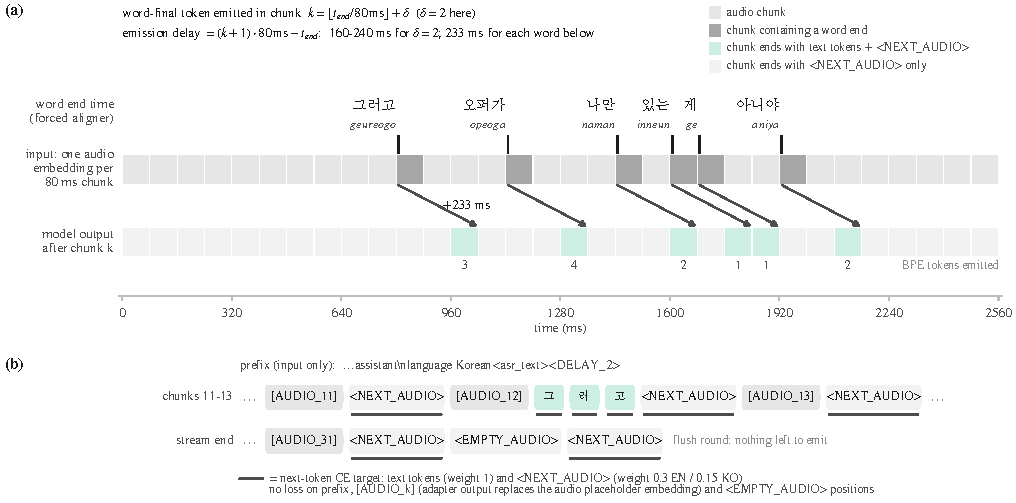
\includegraphics[width=\textwidth]{figures/figA7_delta_delay.pdf}
  \caption{Delay rule of the single-speaker backbone on a recorded KsponSpeech \citep{bang2020ksponspeech} utterance (2.6\,s, $K=32$ chunks, $\delta=2$). (a)~One audio embedding enters per 80\,ms chunk. A word that ends at $t_{\mathrm{end}}$ (forced alignment) is emitted, with all its BPE tokens, after chunk $k=\lfloor t_{\mathrm{end}}/80\,\mathrm{ms}\rfloor+\delta$, so its emission delay $(k+1)\cdot80\,\mathrm{ms}-t_{\mathrm{end}}$ lies between 160 and 240\,ms for $\delta=2$; here it is 233\,ms for all six words. Numbers under the output row count the BPE tokens emitted. (b)~Serialized LM sequence for chunks 11--13 and the end of the stream. Underlined tokens are next-token targets, weighted 1 for text and 0.3 (English) or 0.15 (Korean) for the end-of-chunk token \mdltok{next} (NEXT\_AUDIO); the prefix, the audio positions and \mdltok{empty} (EMPTY\_AUDIO) carry no loss.}
  \label{fig:delta-delay}
\end{figure}

\paragraph{Targets, loss and decoding.}
Targets are normalised lexical transcripts (lowercase, no punctuation, numbers spelled out). Word end times come from Qwen3-ForcedAligner \citep{shi2026qwen3asr} at 80\,ms resolution, and all tokens of a word are due in the chunk that the delay rule assigns to the word's end; tokens due at or after the last chunk go to the flush round, and tokens due in the same chunk keep their end-time order. Training imposes no limit on the tokens per chunk. On LibriSpeech and KsponSpeech, targets average 0.22 and 0.27 text tokens per chunk, and 75--80\% of the chunks emit only \mdltok{next}; \cref{eq:loss} therefore weights \mdltok{next} by 0.3 (English) or 0.15 (Korean) and every other label, including the planned tags, by 1. The output layer is computed only at labelled positions, which bounds memory on long sequences. Decoding is greedy with a KV cache, with one forward pass per chunk and one per emitted token; it forces \mdltok{next} after 8 tokens in a chunk or $6K+64$ tokens in a stream, runs flush rounds until one is empty (at most 8), and blocks the chat-format, audio, transcript-marker, \mdltok{empty}, speaker and delay tokens. Translation segments will need a higher per-chunk cap.\draftnote{planned} On one H200 GPU, decoding with the 0.6B thinker needs 100--150\,ms per 80\,ms chunk at the 99th percentile, so real time is not yet shown; the 1.7B thinker has not been timed (\cref{tab:ca-latency}). In earlier backbones with the 0.6B thinker, $\delta=2/3/4$ gave a median emission delay $(k+1)\cdot80\,\mathrm{ms}-t$ of about 200/280/360\,ms, which excludes the 80\,ms encoder look-ahead that \cref{sec:model-inference} adds, and at most 0.5\% of English emissions (2--5\% of Korean ones) came 80\,ms or more before their target chunk; the evaluation of the 1.7B pilot recorded no emission delays. \Cref{fig:delta-delay} shows the rule on a 2.6\,s utterance: its six words end at 807, 1127, 1447, 1607, 1687 and 1927\,ms and are emitted after chunks 12, 16, 20, 22, 23 and 26, each 233\,ms after its end; chunks 0--11 and 27--31 emit only \mdltok{next}, and the flush round is empty.

\paragraph{Training.}
Stage~0 trains only the adapter, with the thinker frozen, in final mode (the native Qwen3-ASR format), because a randomly initialised adapter otherwise causes very large gradients in the first steps. Stage~1 starts from Stage~0 and the original Qwen3-ASR thinker and trains all parts for one epoch, with $\delta\in\{2,3,4,6,8\}$ and final mode for each utterance with probability 0.3 (\cref{tab:training}). Its data are about 3.8k\,h drawn from a quality-controlled pool of 19 English and Korean sources, plus about 4.3k\,h of ASR corpora: 806\,h of English from LibriSpeech \citep{panayotov2015librispeech}, VoxPopuli \citep{wang2021voxpopuli}, Granary-YODAS \citep{koluguri2025granary} and Switchboard \citep{godfrey1992switchboard}, and about 3.5k\,h of Korean from KsponSpeech \citep{bang2020ksponspeech}, NIKL conversational speech and AI~Hub conversational and broadcast speech; there is no German. We augment with SpecAugment \citep{park2019specaugment} (2 frequency masks of up to 27 bins and 2 time masks of up to 3\% of the utterance), speed perturbation (0.9, 1.0, 1.1), noise (probability 0.4, SNR 5--30\,dB), music (SNR 10--30\,dB) and reverberation (probability 0.2). The noise bank holds 8.9\,h of noise (MUSAN, \citealp{snyder2015musan}; DEMAND, \citealp{thiemann2013demand}; ETSI), 42.6\,h of music (MUSAN) and 6,325 simulated and real room impulse responses; reverberation is applied before noise, and the direct-path peak of each impulse response is aligned to $t=0$ so that word times stay valid. Stronger time masking (about 12\% of the frames) lowered the top-1 accuracy on text tokens at the first step from 0.985 to 0.84, so we avoid it. One epoch takes 3,980 steps on 2 nodes with 8 GPUs each, at about 2.5\,s per step including I/O stalls (0.6--1.0\,s of compute); the training loss ended at 0.27 and was still falling. The 0.6B pilot uses the same data, steps and augmentation. After training, we reload each checkpoint and compare it with the model in memory key by key, encoder included; for both pilots no key differs, including all 638 encoder tensors.
\draftnote{longer Stage-1 runs exist but stay out of the paper until their numbers are recorded with a per-epoch analysis}

% =====================================================================
% Table A11 (tab:training): training stages. Included from App. F.
% Stages 0-1 exist (Stage 1 = the one-epoch pilot behind tab:backbone).
% Stages 2-3 are planned: their Data/Targets cells restate the design of
% Sec. 5 (sec:model); every setting that is still open is \tbd (blank).
% =====================================================================
\begin{table}[t]
  \caption{Training stages, data and hyperparameters. Stages~0 and~1 exist, and the one-epoch Stage-1 pilot is the backbone of \cref{tab:backbone}; Stages~2 and~3 are planned (M1--M3 as in \cref{sec:model}), and their open settings are blank. Hours are approximate; data sources and augmentation are detailed in \cref{app:model}. lr: peak learning rate after a linear warm-up.}
  \label{tab:training}
  \centering
  \footnotesize
  \setlength{\tabcolsep}{2.5pt}
  \renewcommand{\arraystretch}{1.1}
  \begin{tabular}{@{}>{\raggedright\arraybackslash}p{2.1cm}>{\raggedright\arraybackslash}p{1.9cm}>{\raggedright\arraybackslash}p{3.6cm}>{\raggedright\arraybackslash}p{2.9cm}>{\raggedright\arraybackslash}p{3.0cm}>{\raggedright\arraybackslash}p{1.35cm}>{\raggedright\arraybackslash}p{1.1cm}@{}}
    \toprule
    Stage & Trainable & Data & Targets & Schedule & Hardware & Status \\
    \midrule
    0: adapter warm-up
      & adapter (6.3M); thinker frozen
      & English and Korean ASR
      & final mode only (Qwen3-ASR format)
      & 2,000 steps, warm-up 100; 16,384-token batches
      & 1 node
      & built \\
    \addlinespace
    1: streaming and final-mode ASR
      & encoder, adapter, thinker (2,336M)
      & $\approx$3.8k\,h curated English and Korean speech + $\approx$4.3k\,h English and Korean ASR corpora (806\,h English); no German; augmented
      & lexical transcripts; $\delta\in\{2,3,4,6,8\}$; final mode with probability 0.3
      & 1 epoch = 3,980 steps; lr $6{\times}10^{-5}$ thinker (warm-up 500), $10^{-3}$ adapter, $10^{-5}$ encoder
      & 2 nodes $\times$ 8 GPUs
      & built (pilot) \\
    \addlinespace
    2 (M1): two-speaker bilingual ASR
      & \tbd
      & + German ASR, 8\,kHz telephone-band augmentation, simulated two-speaker \pair{En}{De} and \pair{En}{Ko} mono sessions
      & speaker-tagged transcripts at delay $\delta_s$; two-slot speaker activity
      & \tbd
      & \tbd
      & planned \\
    \addlinespace
    3 (M2, M3): translation streams
      & \tbd
      & + CoVoST~2 and MuST-C (\pair{En}{De}); silver teacher translations in four directions
      & translations committed at turn ends (M2) or at MU2 (M3), delay $\delta_t$
      & \tbd
      & \tbd
      & planned \\
    \bottomrule
  \end{tabular}
\end{table}


\paragraph{Planned stages.}
Stage~2 (M1) starts from the 1.7B Stage-1 pilot and adds German ASR data, 8\,kHz telephone-band augmentation, the speaker tags and the activity head, trained on simulated two-speaker \pair{En}{De} and \pair{Ko}{En} mono sessions whose gaps and overlaps are drawn more broadly than in the benchmark \citep[cf.][]{landini2022from}. Each speaker's turns are force-aligned before mixing, so that the words of both speakers can be ordered by end time under overlap (\cref{sec:model-stream}). Before training M1, we fixed three acceptance criteria: single-speaker WER and CER at most 5\% (relative) above those of the Stage-1 pilot on VoxPopuli-AA and KsponSpeech, cpWER on synthetic L0 sessions at most 1.2 times the matched single-speaker WER, and a speaker-attribution error of at most 5\%. Stage~3 then adds the translation streams of \cref{sec:model-targets}, committed at turn ends (M2) or at MU2 (M3), from human \pair{En}{De} speech translation data, CoVoST~2 \citep{wang2021covost} and MuST-C \citep{digangi2019must}, and from silver teacher translations in four directions. The same-backbone cascade and the decoupled twin of \cref{sec:exp-ablation} also start from M1 and train on the same data (\cref{app:baselines}). Unlike the off-the-shelf baselines, \model and both controls thus train on simulated sessions built like the benchmark's; the fixed-gap sweep (\cref{fig:gap-sweep}) tests whether gains depend on the benchmark's gap distribution. Training excludes \taxi, the dialogue corpora and voices of \syn, and outputs of EXAONE-4.0 \citep{lgai2025exaone4}, which serves only for evaluation (\cref{app:syn,app:units}).
\draftnote{planned; German data still has to be obtained, and if M1 misses the criteria twice, M1 transcripts translated by an LLM become our system}

\paragraph{Evaluation protocol.}
Backbone results use a single-turn protocol: each utterance is followed by 1\,s of digital silence, the state is reset per utterance, and decoding is greedy in fp32 with TF32 disabled. English is scored by WER and Korean by CER without spaces, after normalising the text with numbers spelled out. VoxPopuli-AA is a cleaned release of the VoxPopuli test set \citep{wang2021voxpopuli} (628 utterances, 1.98\,h, 292 sessions, 18,072 reference words); AA-WER approximates the scoring published with it, part of which is not public: we apply Whisper's text normalisation \citep{radford2023robust}, split digits and weight the mean by utterance duration. KsponSpeech \citep{bang2020ksponspeech} eval\_clean and eval\_other have 3,000 and 2,687 utterances. Paired bootstrap tests use 2,000 resamples, clustered by session on VoxPopuli-AA and by utterance on KsponSpeech; we call a difference significant if its 95\% interval excludes zero. Differences and relative changes are computed from unrounded error rates.

% =====================================================================
% Table A9 (tab:backbone): single-speaker streaming ASR backbone. Included from App. F.
% All values are measured on the single-turn protocol: the two one-epoch
% Stage-1 pilots, two earlier 0.6B models and two references. Single-speaker
% English and Korean transcription only: these are not CST results.
% Do NOT add the three-epoch Stage-1 runs until their numbers are recorded.
% =====================================================================
\begin{table}[t]
  \caption{Streaming ASR backbone on single-speaker English and Korean speech (not \task): error rates in \% at decoder delay $\delta=4$ and $\delta=6$ and in final mode, encoder context $[56,0]$, single-turn protocol. WER on English VoxPopuli-AA, together with AA-WER, our approximation of the scoring rules published with this test set; CER without spaces on KsponSpeech eval\_clean and eval\_other. $^\ast$Backbone of \model. The two Stage-1 models share data, steps and augmentation (\cref{tab:training}); the earlier 0.6B models are described in \cref{app:model}. Qwen3-ASR-1.7B is non-causal and transcribes whole utterances; the RNN-T is the released Nemotron~3.5 model (the encoder we start from, with its own causal transducer decoder). Both have one operating point. VoxPopuli-AA is not speaker-disjoint from our training data: 80 of its 207 speakers and 280 of its 292 sessions also occur in training. Paired-bootstrap comparisons are given in the text. --: no final mode.}
  \label{tab:backbone}
  \centering
  \footnotesize
  \setlength{\tabcolsep}{3.5pt}
  \begin{tabular}{@{}lcccccccccccc@{}}
    \toprule
    & \multicolumn{3}{c}{VoxPopuli-AA WER} & \multicolumn{3}{c}{VoxPopuli-AA AA-WER} & \multicolumn{3}{c}{Kspon clean CER} & \multicolumn{3}{c}{Kspon other CER} \\
    \cmidrule(lr){2-4}\cmidrule(lr){5-7}\cmidrule(lr){8-10}\cmidrule(l){11-13}
    Model & $\delta=4$ & $\delta=6$ & final & $\delta=4$ & $\delta=6$ & final & $\delta=4$ & $\delta=6$ & final & $\delta=4$ & $\delta=6$ & final \\
    \midrule
    Stage~1, 1.7B thinker$^\ast$   & 7.70 & 7.18 & 6.84 & 5.73 & 5.20 & 4.77 & 9.70  & 9.40  & 8.21 & 9.95  & 9.63  & 8.42 \\
    Stage~1, 0.6B thinker          & 7.73 & 7.18 & 7.14 & 5.73 & 5.09 & 5.09 & 10.55 & 10.24 & 9.27 & 10.87 & 10.47 & 9.22 \\
    Earlier recipe, 0.6B           & 8.94 & 8.01 & --   & 7.18 & 6.16 & --   & 12.32 & 11.76 & --   & 12.86 & 12.67 & --   \\
    Earlier + commit tokens, 0.6B  & 9.88 & 9.15 & --   & 8.02 & 7.26 & --   & 12.26 & 12.04 & --   & 12.26 & 12.19 & --   \\
    \midrule
    Qwen3-ASR-1.7B, offline        & \multicolumn{3}{c}{5.10} & \multicolumn{3}{c}{3.22} & \multicolumn{3}{c}{8.92}  & \multicolumn{3}{c}{8.71}  \\
    Nemotron RNN-T, $[56,0]$       & \multicolumn{3}{c}{6.88} & \multicolumn{3}{c}{4.88} & \multicolumn{3}{c}{19.46} & \multicolumn{3}{c}{16.80} \\
    \bottomrule
  \end{tabular}
\end{table}

\begin{figure}[htbp]
  \centering
  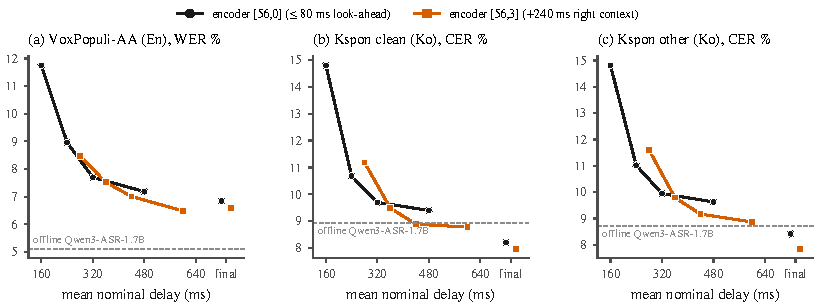
\includegraphics{figures/figA6_backbone_lookahead.pdf}
  \caption{Encoder look-ahead versus decoder delay in the streaming backbone (Stage-1 pilot, 1.7B thinker): error rate against mean nominal delay with encoder context $[56,0]$ (look-ahead ${\le}\,80$\,ms; black circles) and $[56,3]$ (240\,ms more right context; vermillion squares) for $\delta=2,3,4,6$, and in final mode; dashed: offline Qwen3-ASR-1.7B. (a)~VoxPopuli-AA WER (English); (b)~KsponSpeech eval\_clean and (c)~eval\_other CER (Korean). The nominal delay is $80\delta$\,ms for $[56,0]$ and $80\delta+120$\,ms for $[56,3]$. One checkpoint, trained with sampled encoder contexts, is evaluated at both settings. At matched mean delay, encoder look-ahead and decoder delay are largely interchangeable.}
  \label{fig:backbone}
\end{figure}

\paragraph{Backbone results.}
\Cref{tab:backbone} compares the two Stage-1 pilots with two earlier 0.6B models and two references. The earlier recipe trained a 0.6B model in several stages on 5.6k\,h of English and Korean ASR data with $\delta\in\{2,3,4,6\}$ and without final mode; the second earlier model fine-tunes it with sentence-level commit tokens while the encoder is frozen. At $\delta=4$ and $\delta=6$, the 1.7B pilot improves on these two models by 10--24\% and 19--22\% (relative), all significant; only at $\delta=2$ on KsponSpeech is the commit-token model better, by 0.7--1.0 points. Against the 0.6B pilot, the 1.7B thinker is 6--11\% better in every Korean comparison, on par in English streaming, and 4\% better in English final mode (6.84 vs.\ 7.14\%; difference $-0.31$ points, 95\% CI $[-0.57,-0.03]$). Against the released Nemotron~3.5 model at $[56,0]$ (the encoder we start from, with its own causal RNN-T decoder), the English gap closes as $\delta$ grows: $+4.87$ points (+70.8\%) at $\delta=2$, $+0.82$ (+12.0\%) at $\delta=4$, $+0.30$ (n.s.) at $\delta=6$ and $-0.04$ (n.s.) in final mode. On KsponSpeech, the backbone is 24.0\% ($\delta=2$) to 57.8\% (final mode) better on eval\_clean and 11.9\% to 49.9\% better on eval\_other. In final mode, it beats offline Qwen3-ASR-1.7B on KsponSpeech eval\_clean (8.21 vs.\ 8.92\%; $-0.71$ points, $[-1.05,-0.37]$), matches it on eval\_other (8.42 vs.\ 8.71\%, n.s.) and trails it in English by 1.73 points (6.84 vs.\ 5.10\%, +33.9\%).

\paragraph{Caveats.}
These are single-speaker results. VoxPopuli-AA is not speaker-disjoint from our training data, because the official VoxPopuli split is not: 80 of its 207 speakers and 280 of its 292 sessions also occur in training, although no utterance or sentence is duplicated. AA-WER only approximates the published scoring. The final-mode gain over offline Qwen3-ASR on KsponSpeech may be an in-domain effect, since the KsponSpeech training set is part of our data. The training data contain no German, and the backbone has not been evaluated on telephone-band \taxi speech or on two-speaker mixtures, so none of these numbers carries over to \task.

\paragraph{Encoder look-ahead versus decoder delay.}
Latency can be bought with encoder right context or with decoder delay. As the 1.7B pilot was trained with sampled contexts, we evaluate the same checkpoint at $[56,0]$ and $[56,3]$ (\cref{fig:backbone}) and compare the two at their mean nominal delay: $80\delta$\,ms for $[56,0]$ and $80\delta+120$\,ms for $[56,3]$, whose explicit right context adds 120\,ms on average and 240\,ms at most. Below, a difference is the error of $[56,3]$ minus that of $[56,0]$ in points, given as VoxPopuli-AA WER\,/\,KsponSpeech eval\_clean CER\,/\,eval\_other CER, with significance from the paired bootstrap. Between 240 and 320\,ms the evidence is mixed: $[56,3]$ at $\delta=2$ (280\,ms) is better in English than $[56,0]$ at $\delta=3$ (240\,ms) but worse in Korean ($-0.49/+0.51/+0.58$, all significant), and worse everywhere than $[56,0]$ at $\delta=4$ (320\,ms; $+0.77/+1.49/+1.65$, all significant). Between 320 and 480\,ms the two are interchangeable: $[56,3]$ at $\delta=3$ (360\,ms) differs from $[56,0]$ at $\delta=4$ (320\,ms) by $-0.18/-0.21/-0.14$ and from $[56,0]$ at $\delta=6$ (480\,ms) by $+0.34/+0.09/+0.17$, none significant. Right context helps from 440\,ms on ($[56,3]$ at $\delta=4$ vs.\ $[56,0]$ at $\delta=6$: $-0.17$ (n.s.)$/-0.51/-0.46$; at equal $\delta=6$, i.e.\ 600 vs.\ 480\,ms: $-0.70/-0.62/-0.76$, significant) and in final mode ($-0.25/-0.25/-0.58$, all significant), and matching the maximum rather than the mean delay would shrink these gains further. We therefore keep the causal $[56,0]$ and let $\delta$ set the latency, which \model conditions separately for each stream.

